\begin{figure*}
  \begin{subfigure}[b]{0.32\textwidth}
    \centering
    \caption{Random}
    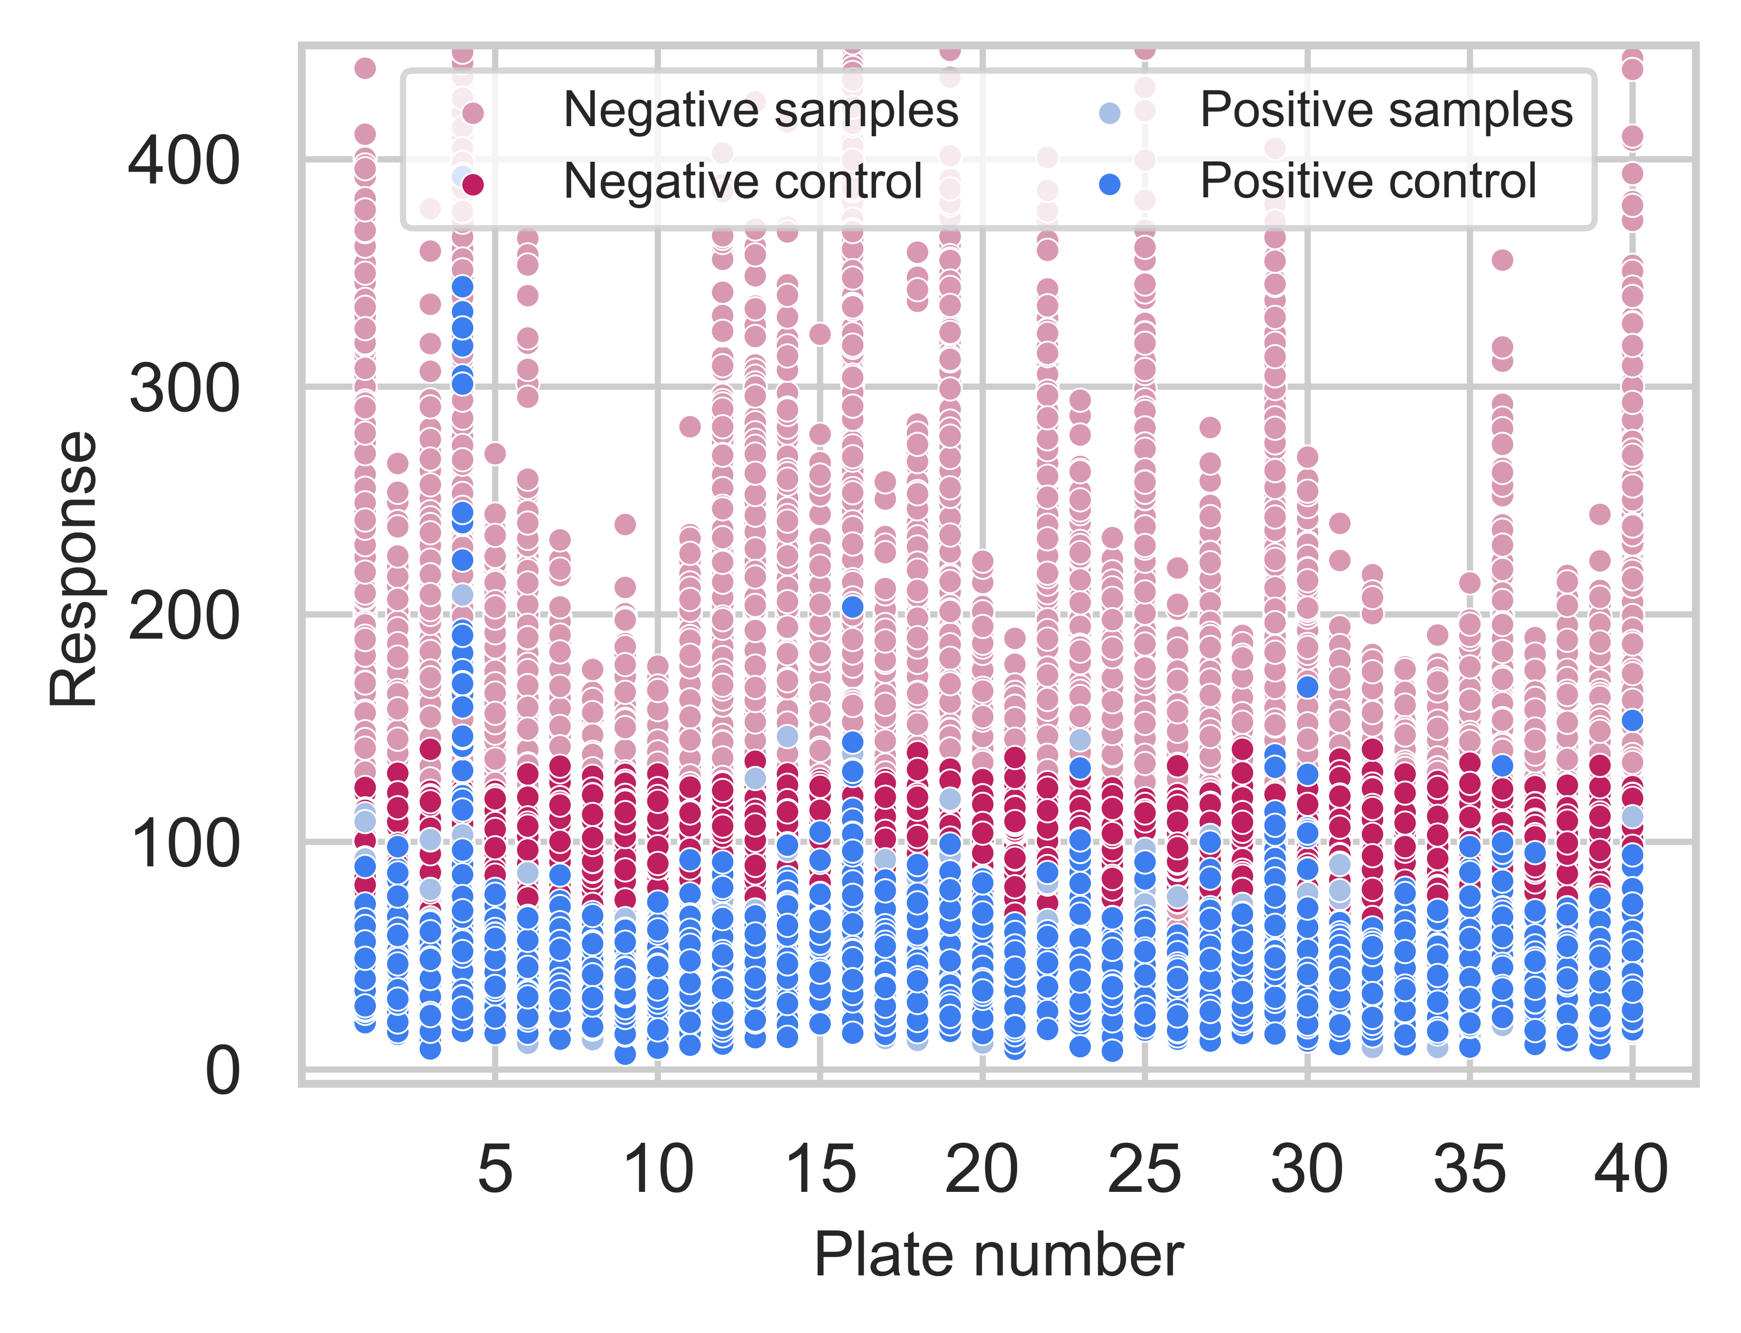
\includegraphics[width=\textwidth]{figures/screening-bowl-0.06-10-10-0.99-stdev-3-4-random.png}
    \label{fig:screen-data-random}
  \end{subfigure}    
  \hfill
  \begin{subfigure}[b]{0.32\textwidth}
    \centering
    \caption{PLAID}
    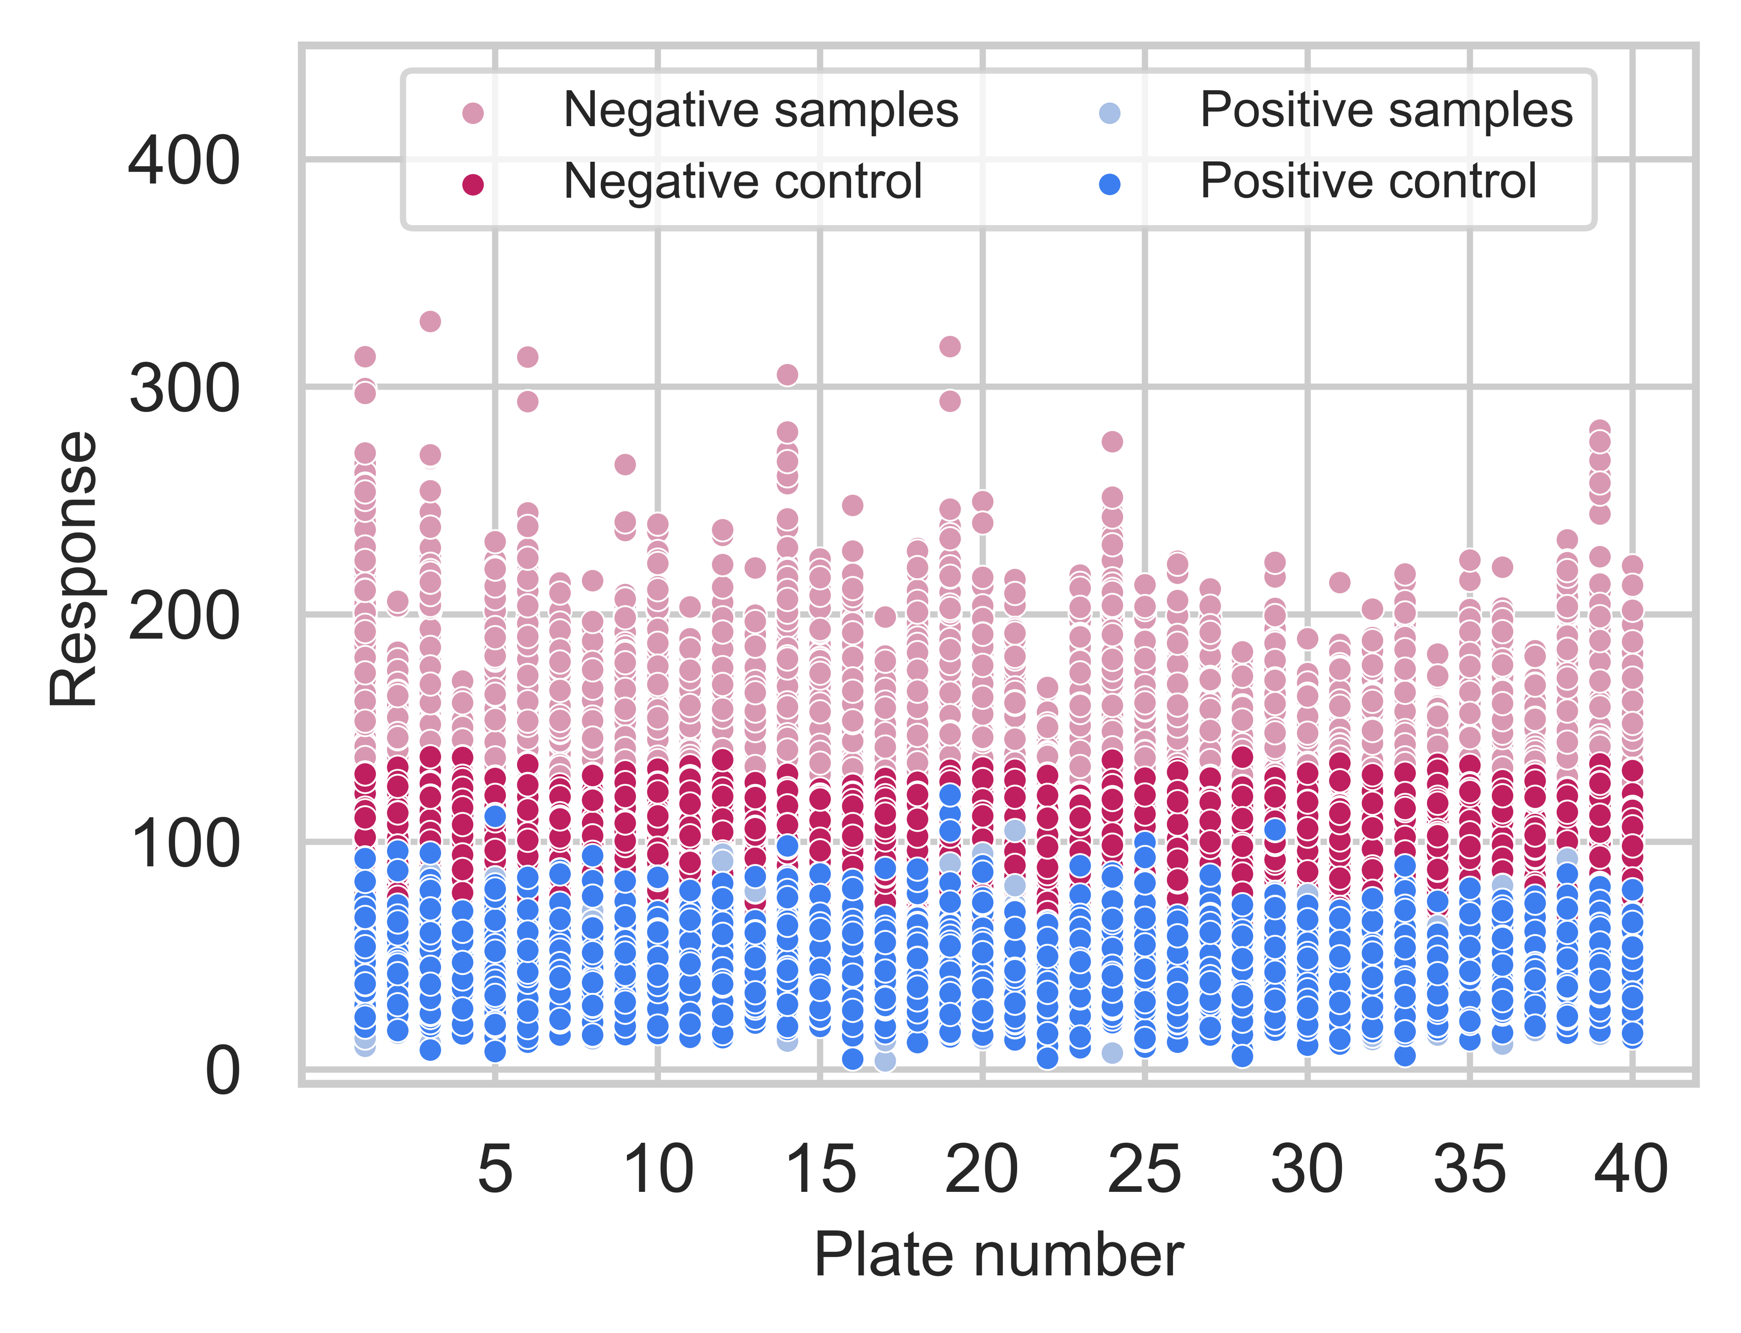
\includegraphics[width=\textwidth]{figures/screening-bowl-0.06-10-10-0.99-stdev-3-4-plaid.png}
    \label{fig:screen-data-plaid}
  \end{subfigure}
  \hfill
  \begin{subfigure}[b]{0.32\textwidth}
    \centering
    \caption{COMPD}
    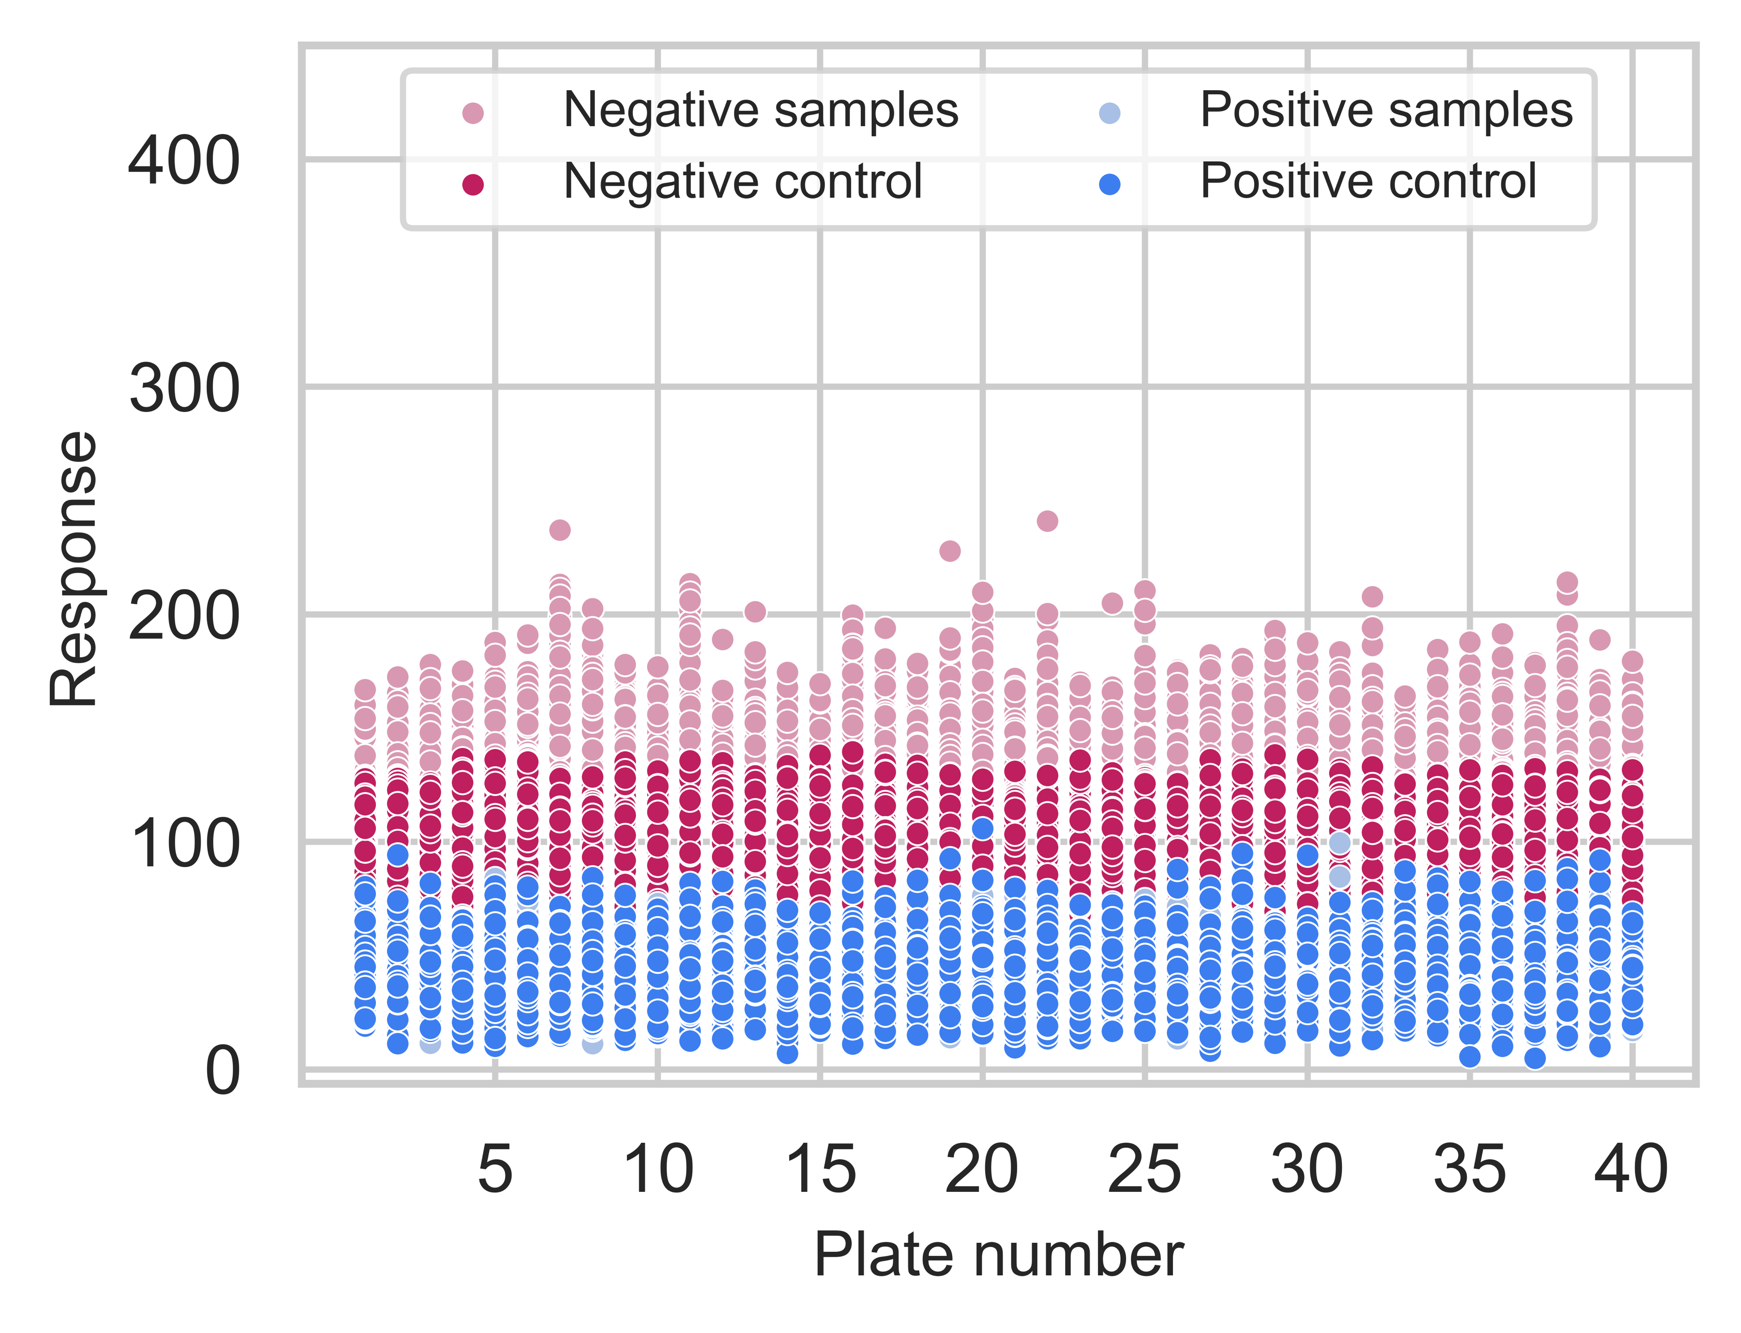
\includegraphics[width=\textwidth]{figures/screening-bowl-0.06-10-10-0.99-stdev-3-4-compd.png}
    \label{fig:screen-data-compd}
  \end{subfigure}

  
  \begin{subfigure}[b]{0.49\textwidth}
    \centering
    \caption{Z' factor}
    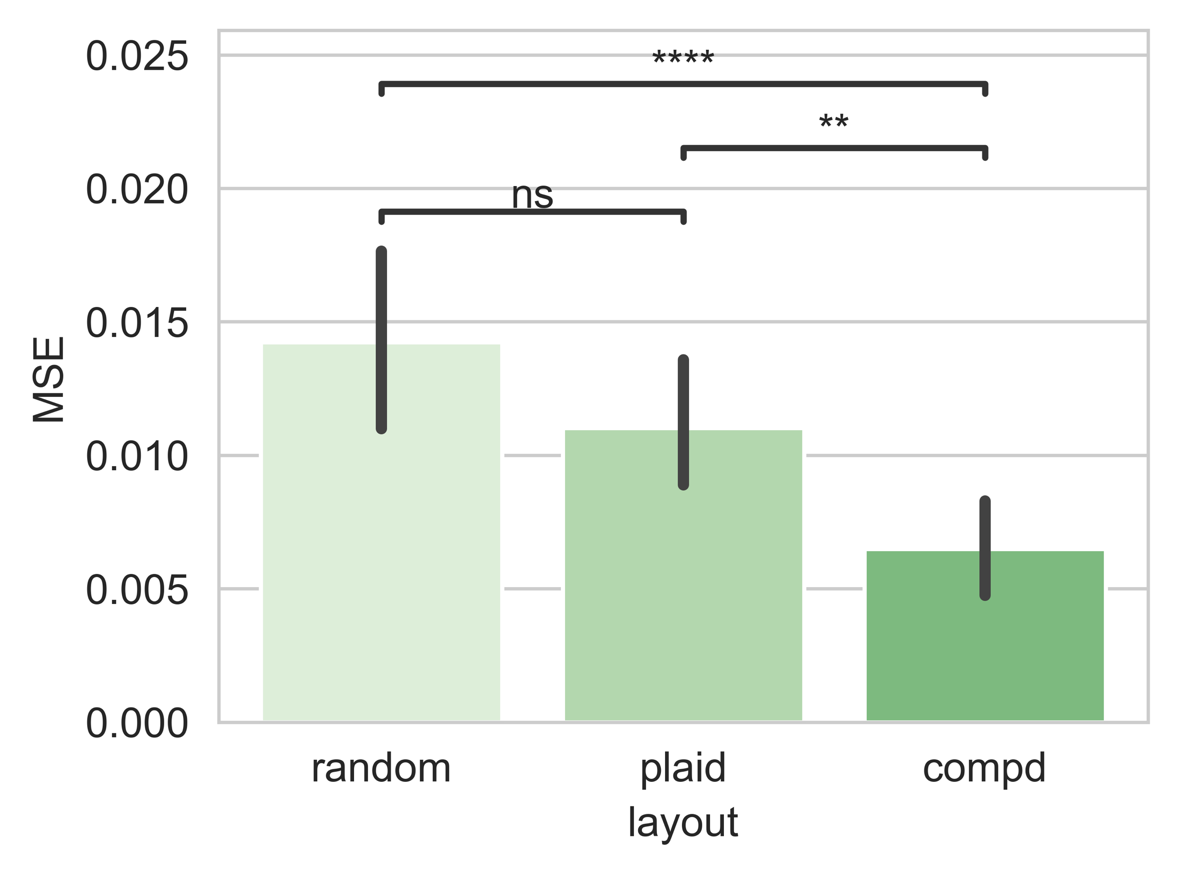
\includegraphics[width=\textwidth]{figures/screening-Zfactor-mse-manuscript.png}
    \label{fig:zpfactor-mse}
  \end{subfigure}
  \hfill
  \begin{subfigure}[b]{0.47\textwidth}
    \centering
    \caption{SSMD}
    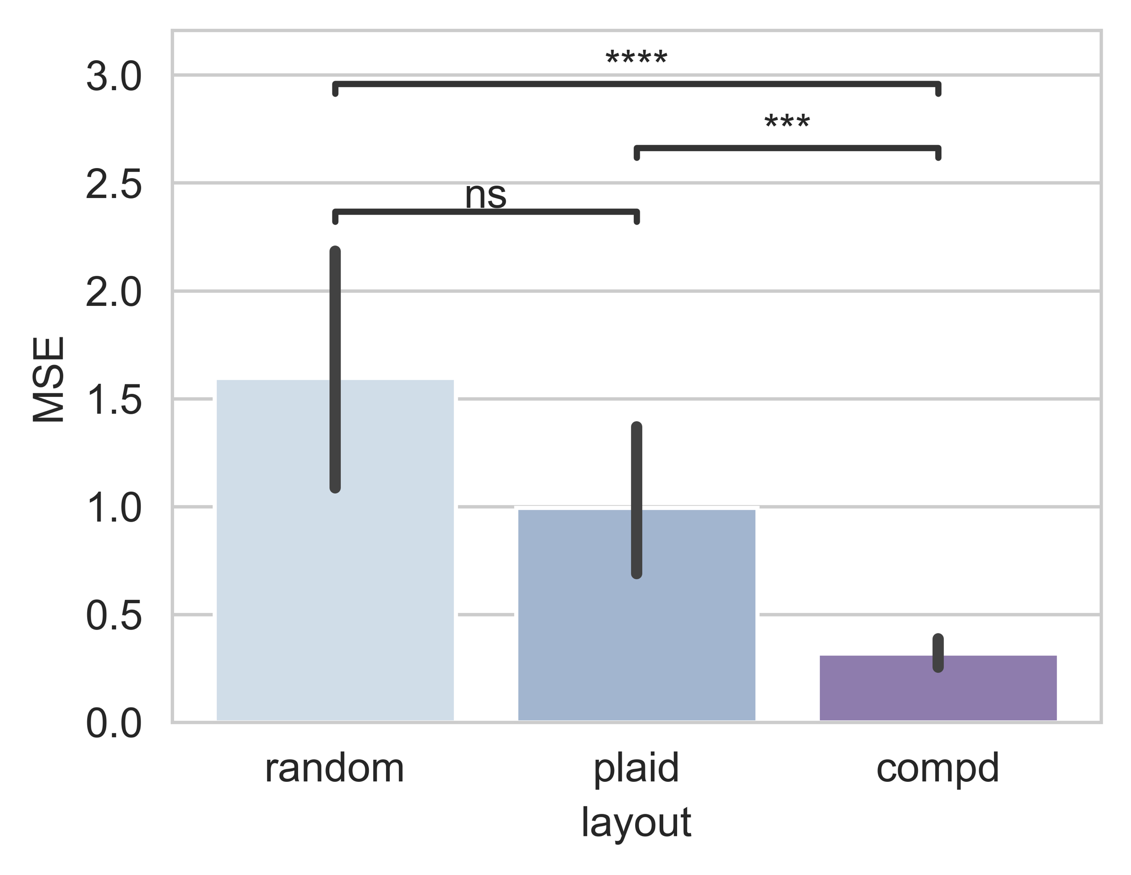
\includegraphics[width=\textwidth]{figures/screening-SSMD-mse-manuscript.png}
    \label{fig:ssmd-mse}
  \end{subfigure}

  
  \begin{subfigure}[b]{0.49\textwidth}
    \centering
    \caption{1\% hits}
    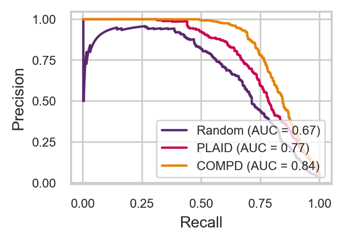
\includegraphics[width=\textwidth]{figures/PR-10-10-0.2-1.png}
    \label{fig:screening-pr-10-10-1}
  \end{subfigure}
  \hfill
  \begin{subfigure}[b]{0.49\textwidth}
    \centering
    \caption{5\% hits}
    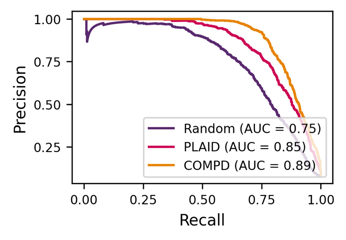
\includegraphics[width=\textwidth]{figures/PR-10-10-0.2-5.png}
    \label{fig:screening-pr-10-10-5}
  \end{subfigure}
  
  
  \caption{Screening experiments consisting of 40 microplates for each type of layout, each
    with 10~positive and 10~negative controls and only
    1~replicate per compound. 
    %
    Hits are randomly distributed on each plate.  %
  %
  (a)-(c):~Simulated response data with 1\% hit rate after error correction and normalisation in the presence of mild bowl-shaped plate effects.
  %
    MSE between expected and obtained (d)~Z'~factor and (e)~SSMD in the presence of mild bowl-shaped plate effects. The expected
      values were calculated using plates randomly filled with 50\% positive controls and 50\% negative controls, constituting the optimal values obtainable by these metrics.
  %
  (f) and (g):~PR (precision recall) curves for experiments with
    varying hit rates in the presence of strong bowl-shaped plate
    effects. }
    \label{fig:screening}
\end{figure*}




%%% Local Variables: 
%%% mode: latex
%%% TeX-master: "main.tex"
%%% End: 
